\chapter{Results}
\thispagestyle{plain}
\label{Results}

\section{Malware Detection}
\label{Malware Detection}

\begin{table}[!htbp]
\caption{Malware Detection Results for Test Set}
\label{malware_binary_detection_test}
\bigskip
\centering
\begin{center}
\begin{tabular}{|c|c|c|c|c|c|c|c|}
\hline
Model & Accuracy & Precision & Recall & F-measure & Specificity  \\ \hline
SdA & 0.996	& 0.9231 & 1 & 0.96	& 0.9958 \\ \hline
Decision Tree & 0.972 & 0.7777	& 0.5833 & 0.6666 & 0.9916 \\ \hline
Ada Boost & 0.976 & 0.875 & 0.5833 & 0.7 & 0.9958 \\ \hline
SVM \(rbf\) & 0.972 & 0.7778 & 0.5833 & 0.6666 & 0.9916 \\ \hline
Random Forest & 0.98 & 1 & 0.5833 & 0.7368 & 1 \\ \hline
Linear & 0.94 & 0.4211 & 0.6666	& 0.5163 & 0.9538\\ \hline
Neural Net & 0.976	& 0.75	& 0.75	& 0.75	& 0.9874  \\ \hline
\end{tabular}
\end{center}
\end{table}


\begin{table}[!htbp]
\caption{Malware Detection Results for Overall Data Set}
\label{malware_binary_detection_overall}
\bigskip
\centering
\begin{center}
\begin{tabular}{|c|c|c|c|c|c|c|c|}
\hline
Model & Accuracy & Precision & Recall & F-measure & Specificity  \\ \hline
SdA & 0.9984 & 0.9629 & 1 & 0.9811 & 0.99834  \\ \hline
Decision Tree & 0.9809 & 0.85 & 0.6538 & 0.7391 & 0.995  \\ \hline
Ada Boost & 0.9904 & 0.9545 & 0.8076 & 0.875 & 0.99834  \\ \hline
SVM \(rbf\) & 0.9872 & 1 & 0.6923 & 0.8182 & 1  \\ \hline
Random Forest & 0.992 & 1 & 0.8076 & 0.8936 & 1  \\ \hline
Linear & 0.9729 & 0.6285 & 0.8461 & 0.7213 & 0.9784  \\ \hline
Neural Net & 0.9904 & 0.8846 & 0.8846 & 0.8846 & 0.995  \\ \hline
\end{tabular}
\end{center}
\end{table}

\begin{figure}[!htbp]
\centering
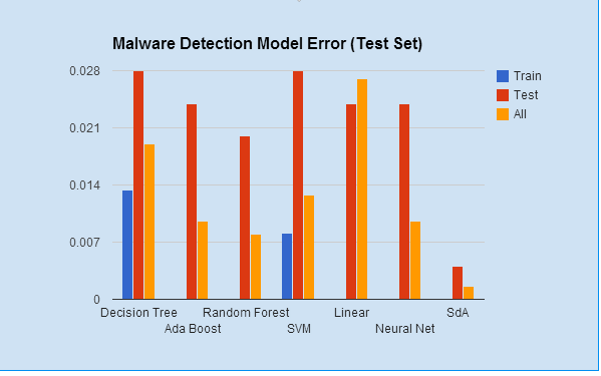
\includegraphics[width=\textwidth, height=0.4\textheight] {binary_model_error}
\caption{Malware detection model error}
\label{fig:malware_detection_err_bar_plot}
\end{figure}

The results of our experiments are shown in the Table~\ref{malware_binary_detection_test} and Table~\ref{malware_binary_detection_overall}. The SdA model has the highest accuracy rate. The model performance increases with increase in number batch size but after 80 batch size the results are stable and we do not get any improvement with performance. Figure~\ref{fig:sda_batch_size_err_rate} shows the performance of SdA model error rate vs batch size. Using spearmint tool we have found optimal values for SdA model. For pre-training and fine-tuning we use 0.01 as a learning rate. We train our model with 200 pre-training epochs and fine-tuning epochs 100. The Figure~\ref{fig:malware_detection_err_bar_plot} shows model error observed for various algorithms.
\begin{figure} [!bp]
\centering
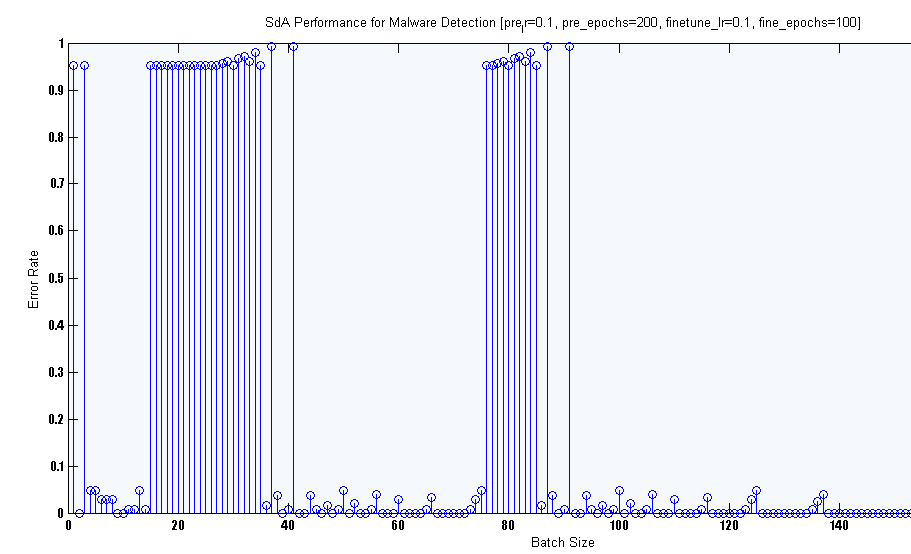
\includegraphics[width=\textwidth, height=0.4\textheight, keepaspectratio] {sda_batch_size_err_rate}
\caption{SdA performance Error rate Vs Batch Size}
\label{fig:sda_batch_size_err_rate}
\end{figure}
The ROC curve analysis testing and overall dataset is shown in Figure~\ref{fig:binary_roc_cureve_test} and Figure~\ref{fig:binary_roc_cureve_all} respectively.

\begin{figure} [!htbp]
\centering
%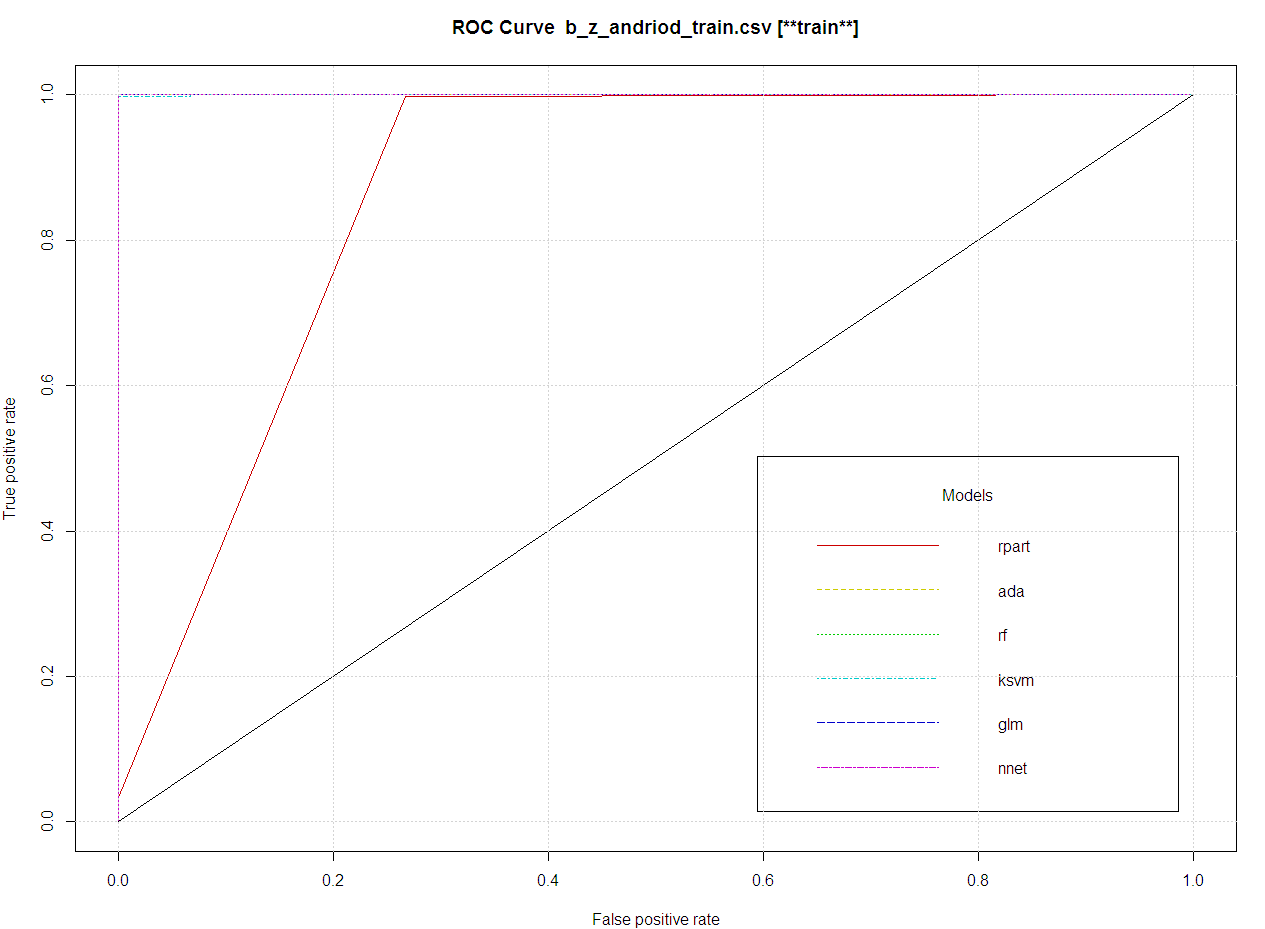
\includegraphics[width=\textwidth, height=0.5\textheight, keepaspectratio] {binary_roc_cureve_train}
%\caption{ROC curve analysis for malware detection models using training data set.}
%\label{fig:binary_roc_cureve_train}
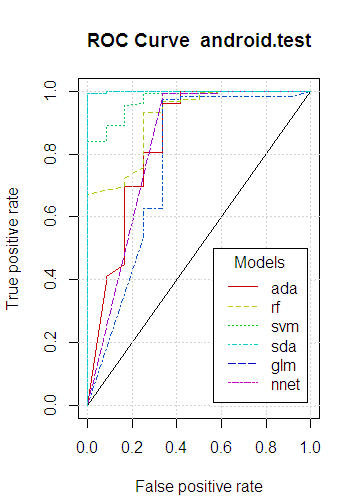
\includegraphics[width=\textwidth, height=0.5\textheight, keepaspectratio] {binary_roc_test_1}
\caption{ROC curve analysis for malware detection models using test data set.}
\label{fig:binary_roc_cureve_test}
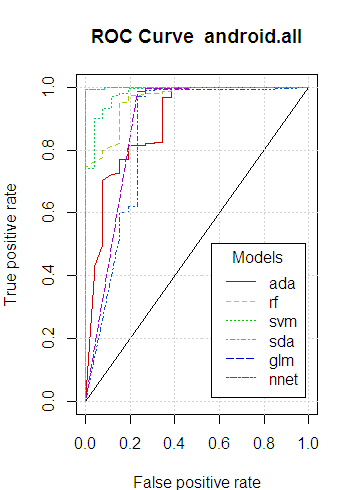
\includegraphics[width=\textwidth, height=0.5\textheight, keepaspectratio] {binary_roc_all_1}
\caption{ROC curve analysis for malware detection models using overall data set.}
\label{fig:binary_roc_cureve_all}
\end{figure}

 
\section{Malware Family Classification}
\label{Malware Family Classification}

\begin{table}[ht]
\caption{AdaBoost, Random Forest, SVM , SdA model's accuracy for malware family classification}
\label{model_accuracy_table}
\bigskip
\centering
\begin{center}
\begin{tabular}{|c|c|c|c|}
\hline
Model	& Train	& Test	& All \\ \hline
AdaBoost &	0.9910525	& 0.7014421	& 0.8931112 \\ \hline
randomForest	& 0.9860335	& 0.6723404	& 0.8634812 \\ \hline
SVM\_RBF	& 0.8324022	& 0.6340426	& 0.7576792 \\ \hline
SVM\_REG	& 0.9860335	& 0.4468085	& 0.7730375 \\ \hline
SdA	& 0.833215	& 0.6632455	& 0.7632453 \\ \hline
\end{tabular}
\end{center}
\end{table}

Figure ~\ref{fig:model_accuracy} shows the over all results for malware family classification. In general Adaboost model performs better than other models. Model performance is provided in Table ~\ref{model_accuracy_table}.
\begin{figure}[ht]
\centering
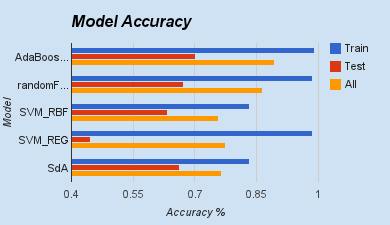
\includegraphics[width=\textwidth, height=0.4\textheight, keepaspectratio]{model_accuracy_graph.png}
\caption{AdaBoost, Random Forest, SVM , SdA model's Accuracy}
\label{fig:model_accuracy}
\end{figure}

\subsection{Randomforest}
We found that random forest algorithm provides best results for forest of 1500 trees. After that results show no marginal improvements over accuracy. Model performance for testing and overall data set is shown in Figure~\ref{fig:rf_test_1500} and Figure~\ref{fig:rf_all_1500} respectively.

\begin{figure}
\centering
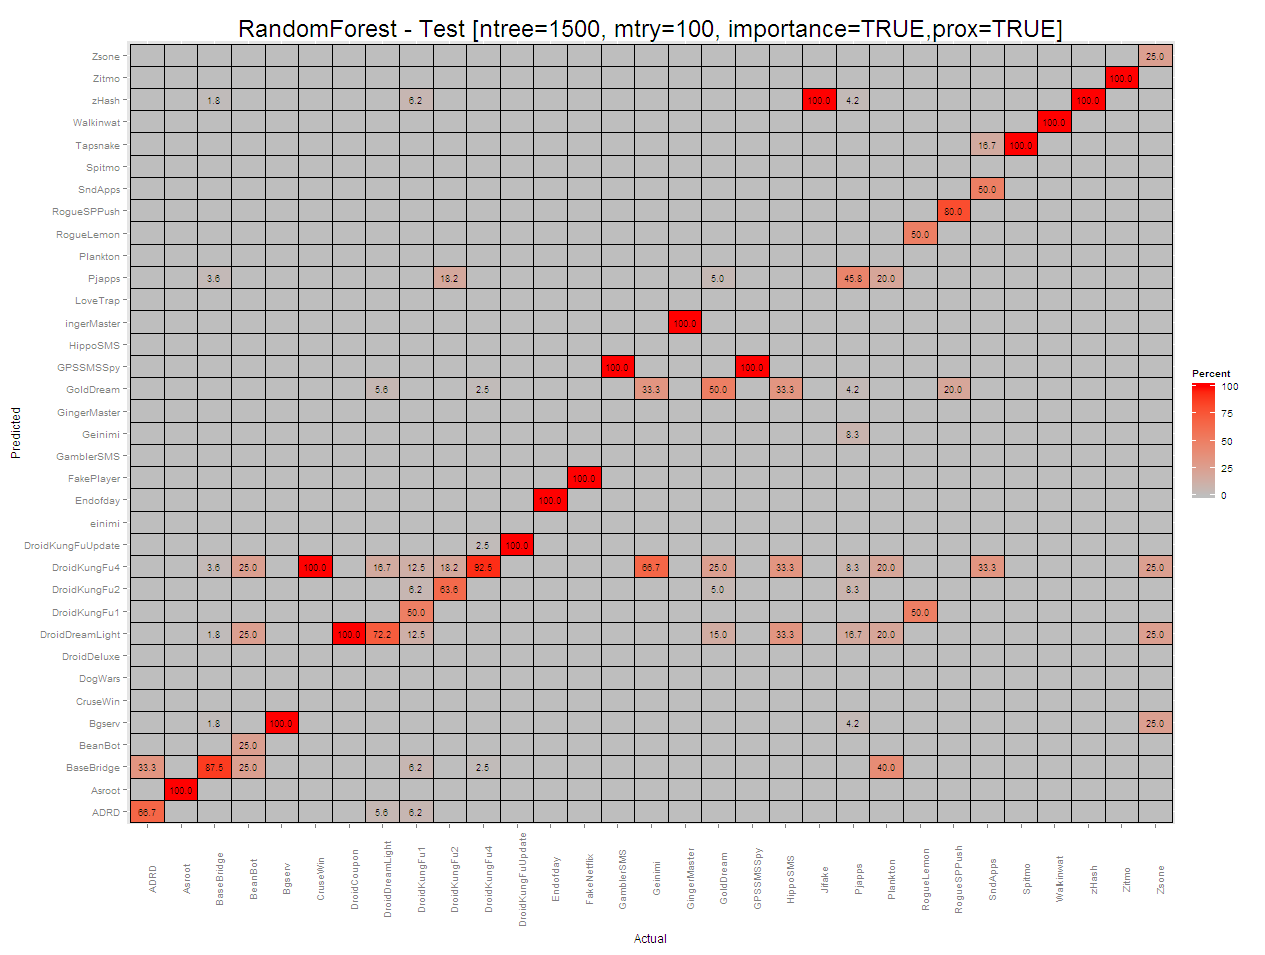
\includegraphics[width=\textwidth, height=\textheight, keepaspectratio] {rf_test_1500}
\caption{Random forest model performance on test data set [ntree=1500, mtry=100, importance=True, prox=True]}
\label{fig:rf_test_1500}
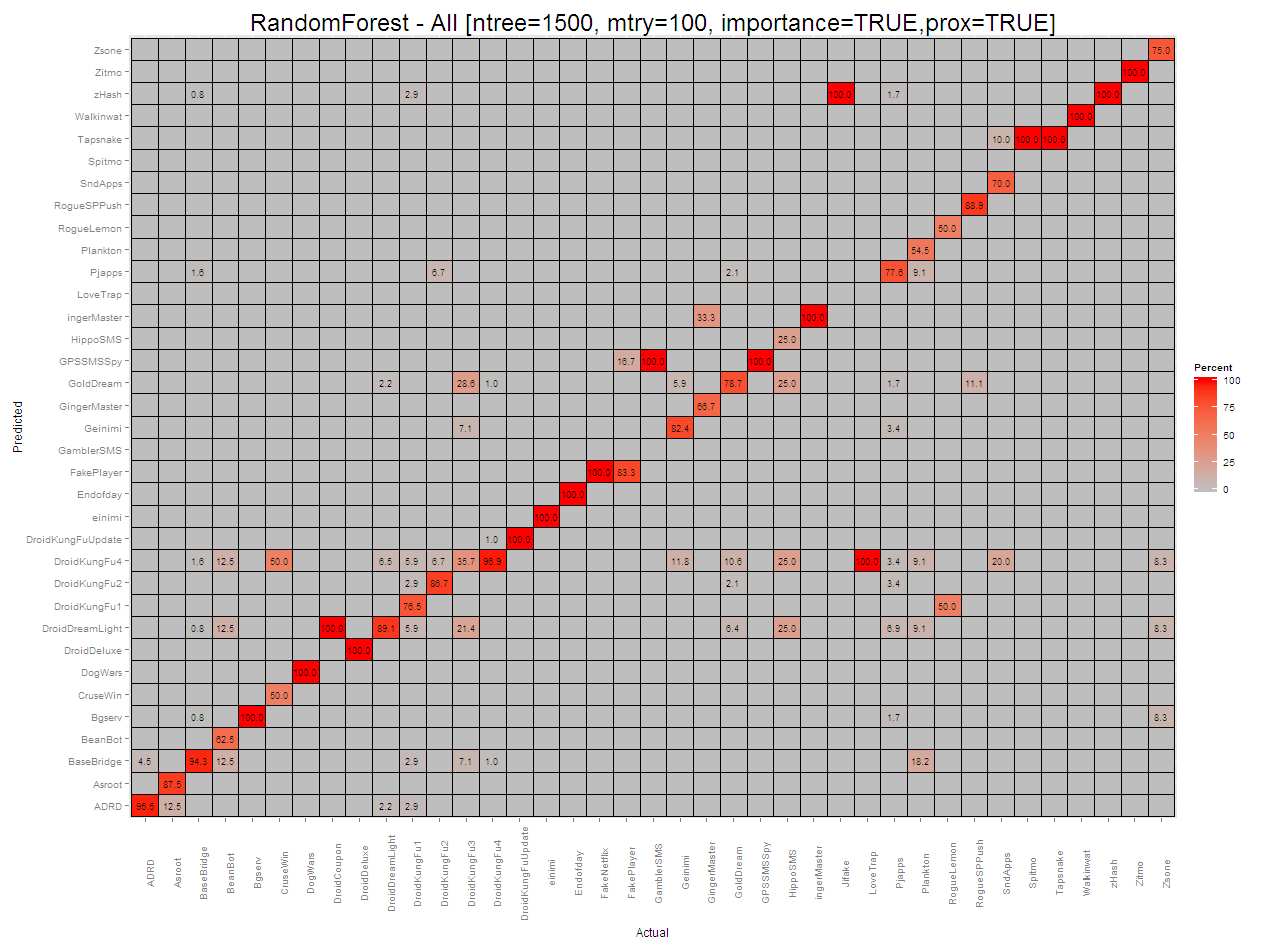
\includegraphics[width=\textwidth, height=\textheight, keepaspectratio] {rf_all_1500}
\caption{Random forest model performance on overall data set [ntree=1500, mtry=100, importance=True, prox=True]}
\label{fig:rf_all_1500}
\end{figure}

\begin{figure}[!htbp]
%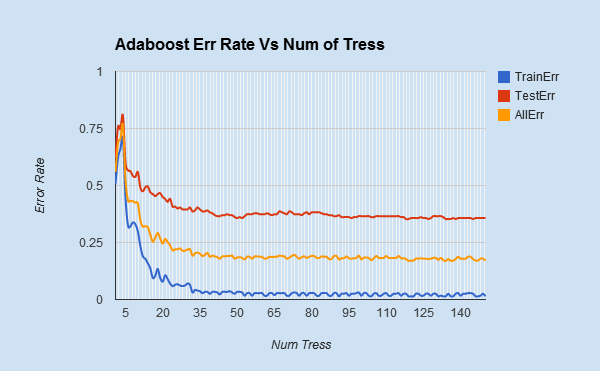
\includegraphics[width=2.72in,height = 4in,keepaspectratio] {adaboost_err_rate}
\centering
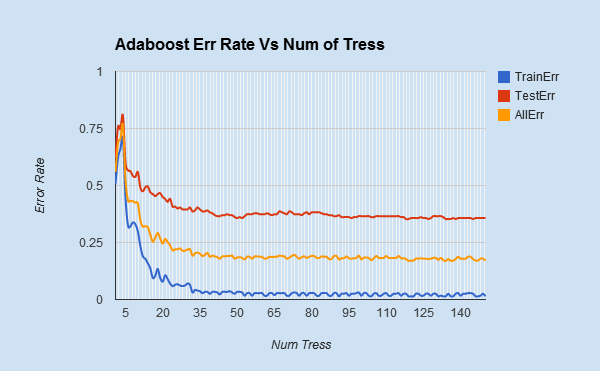
\includegraphics[width=\textwidth, height=0.4\textheight, keepaspectratio] {adaboost_err_rate}
\caption{Performance of Adaboost: Error Rate Vs Num of Trees}
\label{fig:adaboost_err_rate}
\end{figure}

\subsection{AdaBoost}
We use AdaBoost to learn strong classifiers form ensembles of weak learners (decision trees), by varying parameters like minleaf value for the decision trees, the number of iterations for the weak classifier learning and the learning rate. Our aim is to maximize the robustness of the classifier by having fewer and more compact trees. Performance of model for testing and overall data set can is shown in Figure~\ref{fig:adaboost_test} and Figure~\ref{fig:adaboost_all} respectively. The minleaf parameter controls the depth of these tree learners. Our experimental results show that a minleaf value of 30 provides good results for AdaBoost. The boosting model performance increases with increase in number trees but after 50 trees in the results are stable and we do not get any improvement with performance. Figure ~\ref{fig:adaboost_err_rate} shows the performance of AdaBoost model error rate vs. number of tree. Overall both random forest and AdaBoost performs better with malware family classification problem.

\begin{figure}[h]
\centering
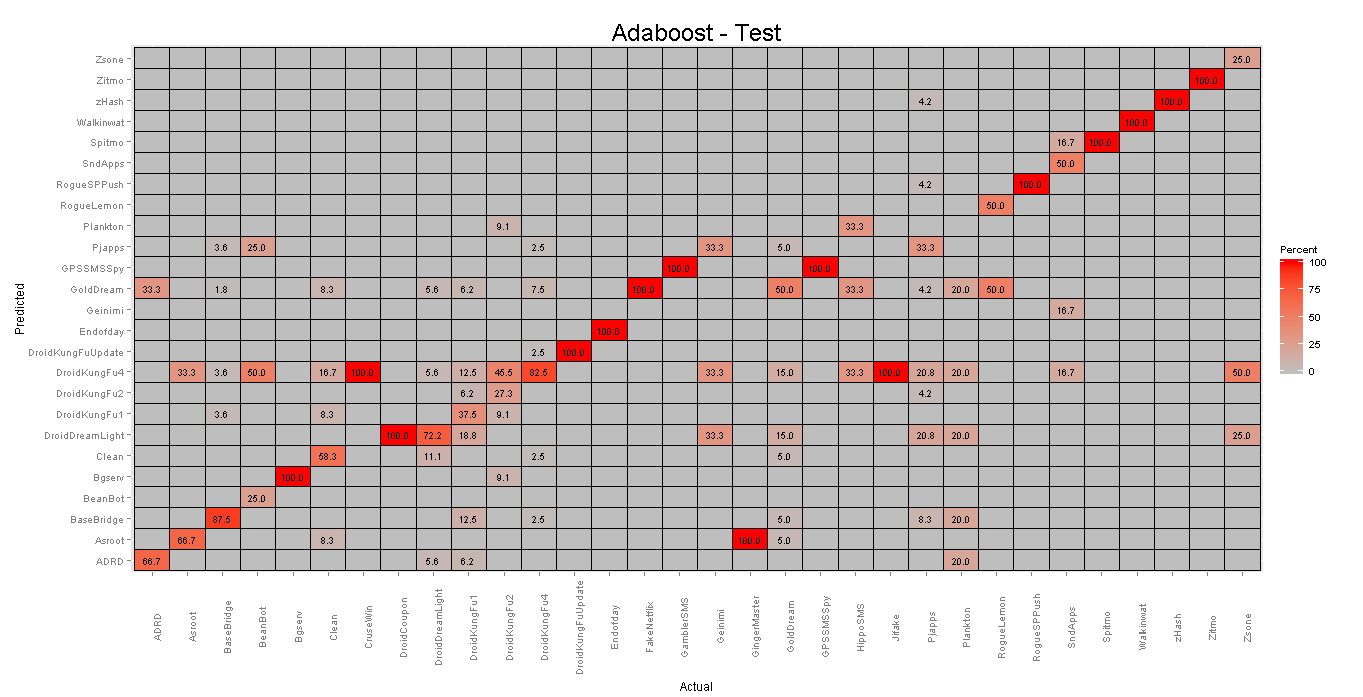
\includegraphics[width=\textwidth, height=0.9\textheight, keepaspectratio] {adaboost_test}
\caption{Adaboost model performance on testing data set for malware family classification}
\label{fig:adaboost_test}
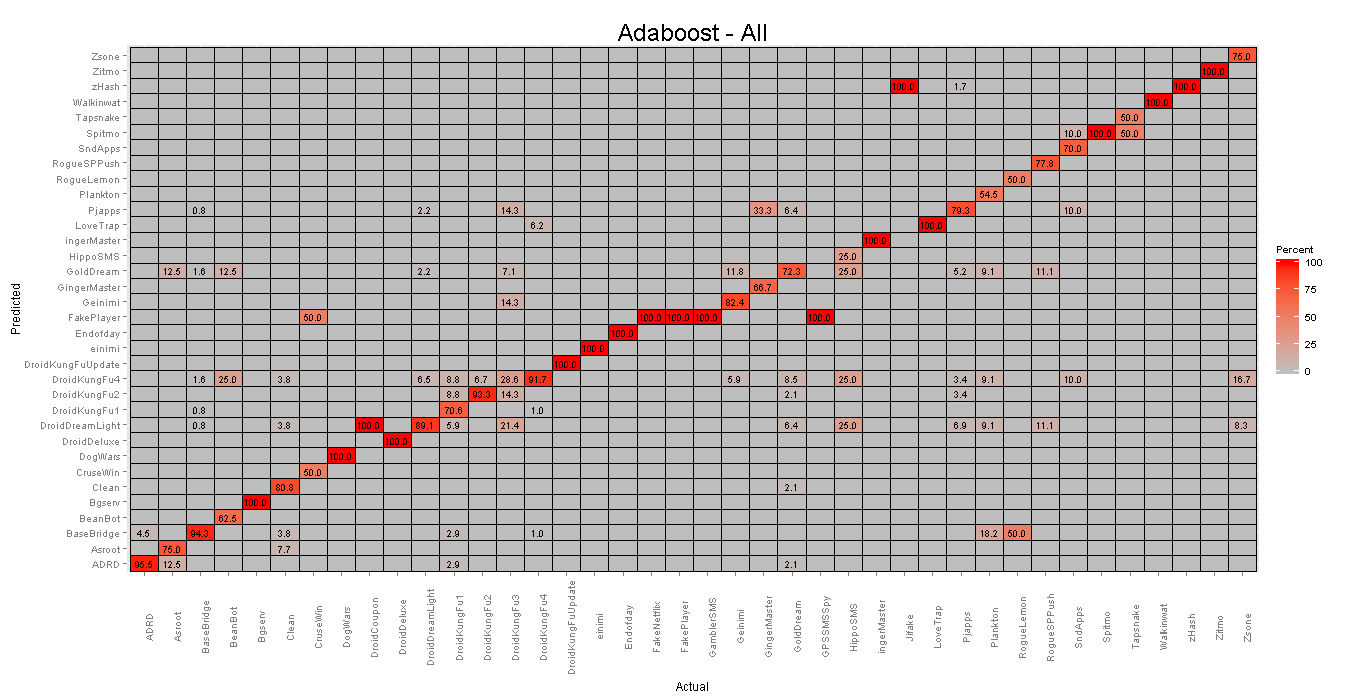
\includegraphics[width=\textwidth, height=1.1\textheight, keepaspectratio] {adaboost_all}
\caption{Adaboost model performance on overall data set for malware family classification}
\label{fig:adaboost_all}
\end{figure}

For AdaBoost algorithm we choose 50 weak learners since minimum number of learners would mean maximum performance. However, experiments are done for different number of learners (n) values - 1, 5, 10, 20, 50 , 100 and 150. It is seen that the values of positive predictive value and accuracy for different number of learners follow an increasing trend for AdaBoost classification. The classifier trees AdaBoost are constructed to see what features are being used while classification. The robustness of the classification techniques is tested by obtaining the features in the classifier trees for different values of n. It is seen that the set of features used by the classifier trees are consistent for the given range of n values. After several runs of experiments we take a suitable value of n = 50 as standard.


\subsection{Support Vector Machine}
We also evaluate the performance of SVM for given dataset. We trained our dataset on SVM machine using rbf kernel. SVM model performs better with rbf kernel for binary classification but provides poor results for malware family classification. Model performance for test and overall dataset is shown in Figure~\ref{fig:svm_rbf_test} and Figure~\ref{fig:svm_rbf_all} respectively.
\begin{figure}
\centering
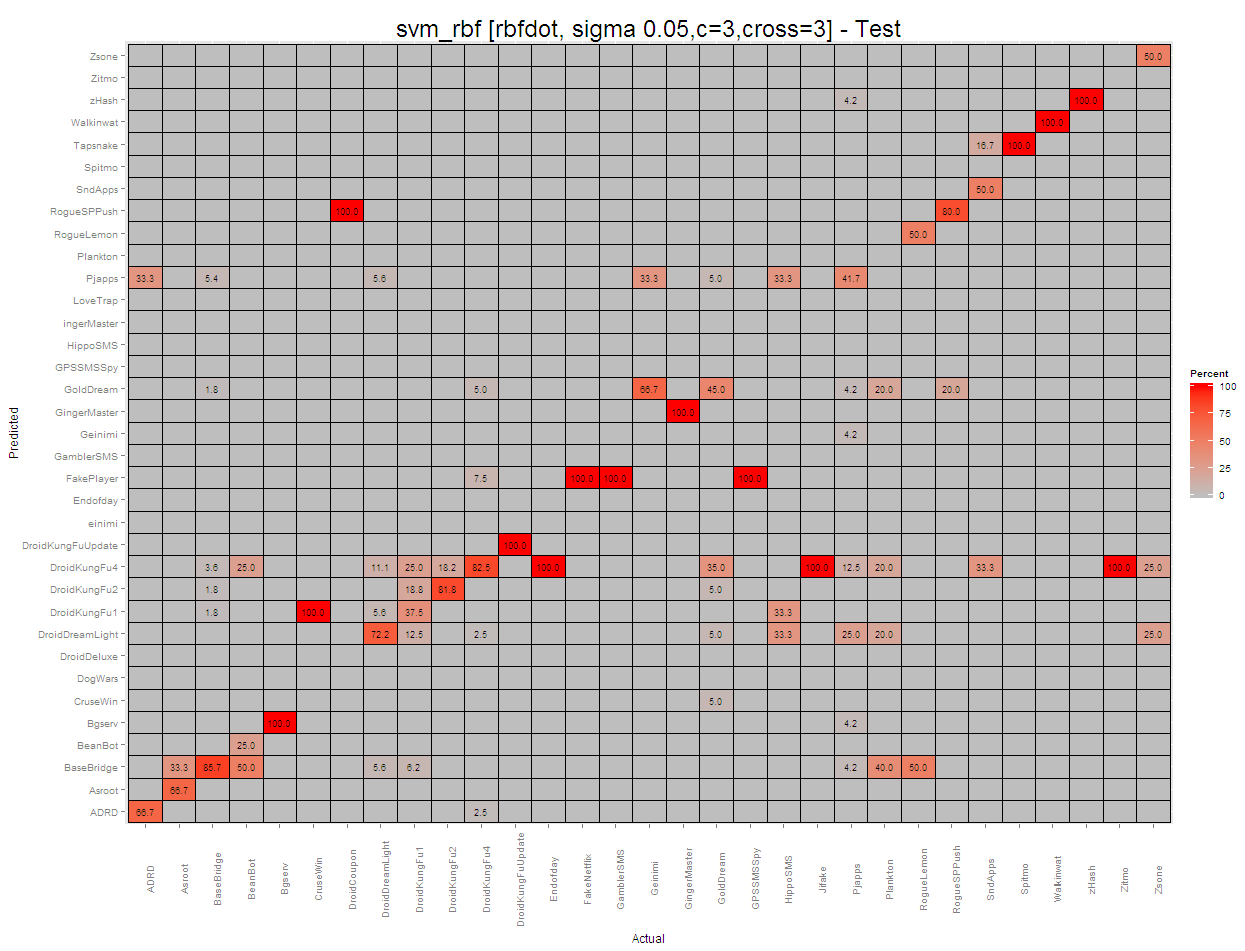
\includegraphics[width=\textwidth, height=0.5\textheight, keepaspectratio] {svm_rbf_test}
\caption{SVM RBF model performance on test data set. [sigma = 0.05, c = 3 , cross = 3]}
\label{fig:svm_rbf_test}
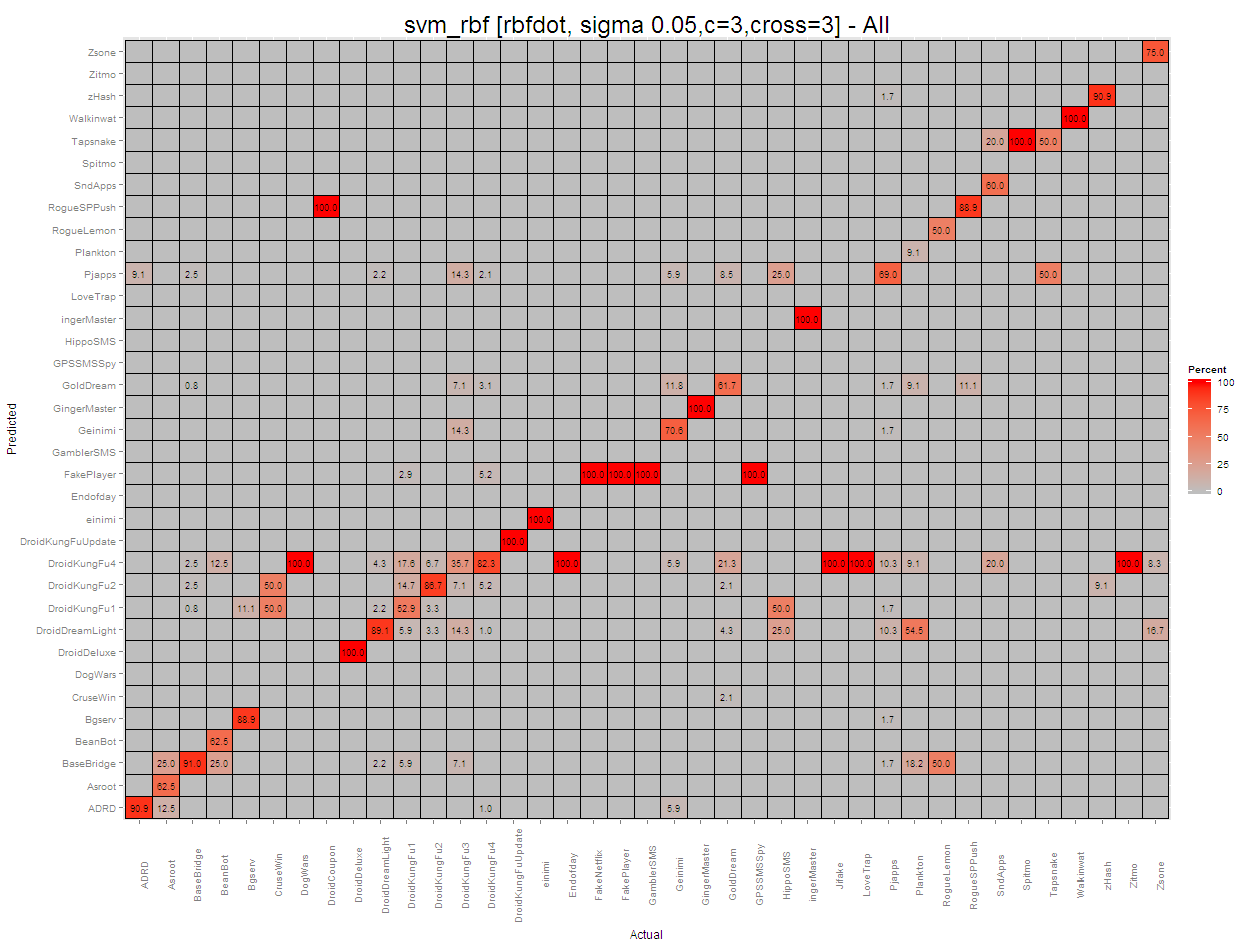
\includegraphics[width=\textwidth, height=0.5\textheight, keepaspectratio] {svm_rbf_all}
\caption{SVM RBF model performance on overall data set. [sigma = 0.05, c = 3 , cross = 3]}
\label{fig:svm_rbf_all}
\end{figure}
